% !TEX encoding = UTF-8
% !TEX program = pdflatex
% !TEX root = guidaconsole.tex

\documentclass[b5paper,11pt,openany]{guidatematica}
\ProvidesFile{guidaconsole.tex}[2014/03/14 v.1.2.3 Guida alla riga di comando]
\GetFileInfo{guidaconsole.tex}

\usepackage{tcolorbox}
\usepackage{guit}% \GuIT
\usepackage{menukeys}
\usepackage{mflogo}
\usepackage{cclicenses}

\definecolor{guitgreen}{rgb}{0,0.5,0}

\tcbset{colback=guitgreen!10,
        colframe=guitgreen,
        fonttitle=\sffamily}

\usepackage[
   colorlinks=true,
   linkcolor=blue,
   citecolor = blue,
   urlcolor = blue,
   pdftitle={Utilizzo della console a riga di comando},
   pdfauthor={Roberto Giacomelli},
   pdfsubject={Guida tematica del GuIT},
   pdfkeywords={console, terminale, riga di comando}
   ]{hyperref}

\frenchspacing

\title{%

\includegraphics[width=0.1\textwidth]{image/terminal-icon}%
\par Guida tematica alla riga di comando}
\author{Roberto Giacomelli}
\date{\filedate{} --- \fileversion}

\begin{document}
\frontmatter
\maketitle

{\Large
Associati anche tu al \GuIT*
\hfill
\keys{\href{http://www.guitex.org/home/it/diventa-socio/associarsi-a-guit}{%
Fai click per associarti}}
}
\medskip

L'associazione per la diffusione di \TeX{} in Italia riconosciuta ufficialmente
in ambito internazionale, si sostiene \emph{unicamente} con le quote sociali.

Se anche tu trovi che questa guida tematica gratuita ti sia stata utile, il mezzo
principale per sdebitarti è diventare socio.
\medskip

Divenendo soci riceverete gratuitamente:
\begin{itemize}
\item
l'abbonamento alla rivista \Ars;
\item
il DVD \TeX{} Collection;
\item
l'esclusivo tipometro realizzato da Massimo Caschili.
\end{itemize}

L'adesione al \GuIT*{} prevede un quota associativa compresa tra 12,00€ e 70,00€
a seconda della tipologia di adesione prescelta ed ha validità per l'anno solare
in corso.

\vfill

\noindent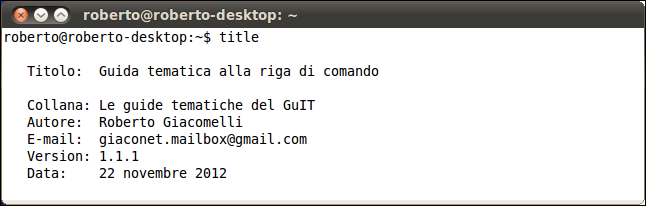
\includegraphics[width=\textwidth]{image/title}

\bigskip
\noindent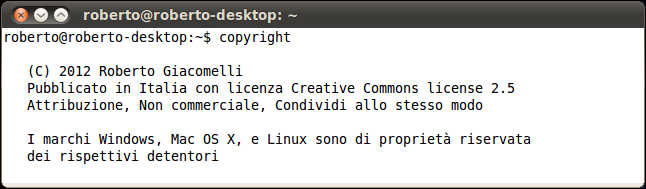
\includegraphics[width=\textwidth]{image/copyright}

\bigskip
\scalebox{1.6}{\cc \ccby \ccnc \ccsa}
\newpage
\tableofcontents
\newpage

% !TEX encoding = UTF-8
% !TEX program = pdflatex
% !TEX root = ../guidaconsole.tex

%
%
%
\chapter{Piano della guida}

Questa guida tematica è suddivisa in quattro sezioni principali:
\begin{enumerate}
\item è una presentazione concettuale della riga di comando sostenuta da accenni
alla sua lunga storia (pagina~\pageref{chapConsole});

\item è un sunto delle particolarità operative di base dell'ambiente di shell
(pagina~\pageref{chapShell});

\item è lo svolgimento passo passo delle procedure per raggiungere le capacità e
le conoscenze necessarie per lavorare autonomamente con la shell di sistema, da
leggere anche indipendentemente dalle altre sezioni (pagina~\pageref{chapEser});

\item è un compendio di argomenti avanzati (pagina~\pageref{chapAvanz}).
\end{enumerate}

La modalità di consultazione dipende dalle conoscenze e dagli obiettivi del
lettore. Probabilmente chi già utilizza la shell sarà interessato ad uno sguardo
sugli aspetti generali ed ad un approfondimento su quelli specifici per
l'utilizzatore \TeX, mentre il neofita potrebbe volersi cimentare subito con
l'indirizzo pratico della terza sezione e sorvolare sui concetti che la
sovrintendono.

Comunque sia, auguro a tutti una buona e spero proficua lettura. Scrivetemi
senza indugio un messaggio di posta elettronica per segnalarmi errori o
miglioramenti o richieste di chiarimenti, e spero mi mandiate le vostre
impressioni, soprattutto se non avevate mai lavorato con la riga di comando
prima d'ora \texttt{:-)} .

\medskip
\hfill\begin{tabular}{c}
Roberto Giacomelli\\
\texttt{giaconet dot mailbox at gmail dot com}\\
\end{tabular}
% eof


\mainmatter

% !TEX encoding = UTF-8
% !TEX program = pdflatex
% !TEX root = ../guidaconsole.tex

\chapter{La riga di comando}
\label{chapConsole}

Prima della comparsa delle interfacce grafiche --- ideate al Palo Alto Research
Center in California ed implementate da Apple prima in Lisa e poi in Macintosh
nel 1983 --- l'interazione con i programmi avveniva con una modalità testuale
chiamata \emph{riga di comando}, ancora oggi disponibile sui moderni elaboratori
come componente essenziale e metodo efficiente di elaborare dati.

I componenti del sistema \TeX{} possono essere utilizzati per mezzo della sola
interfaccia a riga di comando --- ed è per questo che gli utilizzatori
potrebbero avvantaggiarsi se la conoscessero. Ciò non toglie che componenti
indipendenti come gli \emph{shell editor}, possano costituire un'interfaccia
grafica verso i programmi di composizione della famiglia \TeX{}.

\section{Il concetto di base}

\begin{tcolorbox}[title=Definizione di \emph{Riga di comando}]
La \emph{riga di comando} è un ambiente testuale in cui si impartiscono
istruzioni digitando nomi di programmi con eventuali argomenti
\end{tcolorbox}

L'ambiente testuale che consente all'utente di interagire con il sistema è
chiamato \emph{shell}. La shell accetta i dati di ingresso sotto forma di
\emph{comando}, gestisce l'esecuzione ad essi corrispondente e riceve i dati di
uscita destinati all'utente. Nulla vieta che informazioni di ingresso o di
uscita siano memorizzati in file su disco.

La riga di comando ha una lunga storia ed è naturale che le siano stati
attribuiti nomi diversi per definirla nell'ambito di un particolare sistema
operativo --- \emph{linea di comando}, \emph{terminale}, \emph{console} sono fra
questi --- tuttavia i concetti che la definiscono sono ancora quelli
perfezionati da Dennis Ritchie, Ken Thompson, Brian Kernighan e da altri
programmatori esperti dei laboratori Bell sul finire degli anni '60 con Unix.

Tra le innovazioni del sistema operativo Unix, la shell rappresentava l'idea che
piccoli e veloci programmi specializzati in compiti precisi, potessero essere
concatenati in una \emph{pipeline} adottando l'output dell'elaborazione come
input per il programma successivo. La filosofia degli strumenti tende a
garantire lo sviluppo efficiente del software senza limitare la complessità
dell'elaborazione.

Oggi tra i sistemi desktop più diffusi, Mac OS X e Linux, sono basati sulla
struttura di Unix, mentre Windows ha seguito uno sviluppo parallelo replicando
ed ampliando l'ambiente di \textsc{ms-dos} con il ruolo di shell.



\section{Primi comandi}

Il formato delle istruzioni prevede in particolare la digitazione in un'unica
riga del nome del programma, seguito da eventuali opzioni e da eventuali
argomenti. L'esecuzione ha inizio premendo il tasto invio.
\medskip

\texttt{\$ \prog{nomeprogramma} \oarg{opzioni} \oarg{argomenti}}
\medskip

Solitamente le opzioni vengono distinte dai dati premettendo al loro nome uno o
due trattini \texttt{-} oppure uno slash. Se per esempio si vuol conoscere la
versione di un programma è sufficiente eseguirlo con l'opzione
\textsf{-version}. Con \textsf{pdftex}, il principale programma di composizione
del sistema \TeX{}, otteniamo:
\begin{verbatim}
$ pdftex -version
pdfTeX 3.1415926-2.5-1.40.14 (TeX Live 2013)
... eccetera
\end{verbatim}

Nel comando precedente non vi sono argomenti ma solamente un opzione che provoca
la stampa a video di un breve testo contenente le indicazioni di versione del
programma \textsf{pdftex} installato sul sistema. Altri programmi della riga di
comando utilizzano invece altre chiavi per emettere il testo d'aiuto a
dimostrazione che non esiste un unico standard rispettato da comandi o shell.

Se consideriamo l'opzione \texttt{-help} oppure \texttt{-?} si richiederà la
stampa sintetica della sintassi prevista con l'elenco delle opzioni disponibili
e brevi testi esplicativi. Proviamo al terminale:
\begin{verbatim}
$ pdftex -help
Usage: pdftex [OPTION]... [TEXNAME[.tex]] [COMMANDS]
   or: pdftex [OPTION]... \FIRST-LINE
   or: pdftex [OPTION]... &FMT ARGS
... eccetera
\end{verbatim}

Il \texttt{\$} --- o \texttt{>} per i sistemi Windows --- è chiamato
\emph{prompt} ed è il segno dopo il quale si digitano i comandi con il compito
di separare informazioni utili dai comandi stessi. Nella guida faremo uso del
\texttt{\$} riportandolo negli esempi come primo carattere a simboleggiare la
shell.

A volte i comandi possono essere interattivi ovvero, una volta avviati, possono
richiedere ulteriori dati in funzione dell'andamento dell'esecuzione.

\section{Avviare la riga di comando}\label{secAvvio}

Come vedremo, le modalità con cui si opera con la shell non sono poi così
diverse tra i vari sistemi operativi. Molti concetti sono comuni e spesso i
comandi di base hanno addirittura lo stesso nome e già questo è uno spunto di
riflessione interessante.

Solitamente la shell si presenta come una normale finestra grafica --- modalità
detta in emulazione di terminale --- al cui interno compare il cursore
lampeggiante davanti al prompt in attesa di istruzioni.

Nei prossimi paragrafi impareremo ad accedere alla shell in Windows, Mac~OS~X, e
Linux.

\subsection{La shell in Windows}

In Windows la shell è chiamata \emph{Prompt dei comandi}. Vi si accede dalla
barra dei comandi \menu{Start > Programmi > Accessori > Prompt dei comandi}.
Per comodità è possibile creare un shortcut o scorciatoia --- un piccolo file
puntatore ad un altro file --- sul Desktop o nella barra delle applicazioni,
così che basta un click per avviarla.

In Windows esiste una modalità particolare di avvio della shell che consiste
nell'aprire il dialogo \texttt{Esegui...} dal menù Start e digitare il comando
\texttt{cmd} prima di confermare su \keys{OK} o con il tasto \keys{\return}.

\subsection{La shell in Mac OS X}

In Mac la riga di comando è rappresentata dall'applicazione \textsf{Terminale},
situata nella cartella Utility all'interno della cartella Applicazioni.

Potete anche trascinare l’icona Terminale dalla directory Utility di
Applicazioni, alla \emph{Dock Bar}. Per avviare la shell fate click sull'icona
appena creata.

\subsection{I sistemi operativi Linux}

In Linux la shell è di casa. Se il vostro Desktop Environment (DE) è Gnome
utilizzerete \texttt{gnome-terminal} dal menù \menu{Applicazioni > Accessori >
Terminale}. In KDE l'emulatore di terminale è il programma \texttt{Konsole}.

Troverete molto comodo avviare il Terminale da tastiera con una combinazioni di
tasti, per esempio \keys{\ctrl + \Altwin + T}, da impostare nelle scorciatoie
del DE.

In Linux esiste anche il concetto di \emph{console virtuale}, l'insieme di 7
sessioni utente parallele, 6 con interfaccia a caratteri ed una grafica (quella
che utilizziamo normalmente). Si può passare da una all'altra premendo i tasti
funzione da \keys{F1} a \keys{F6} con la combinazione \keys{\ctrl + \Altwin +
F1-6}, per le console a caratteri ed il tasto funzione \keys{F7} nella
combinazione \keys{\ctrl + \Altwin + F7}, per la sessione grafica in cui opera
il Desktop Environment.

Le 6 console testuali sono ambienti a riga di comando di accesso indipendente al
sistema, in cui è necessario eseguire il log-in fornendo un account valido
accreditato sul sistema. Potremo così avviare fino a 7 sessioni parallele
indipendenti sullo stesso computer e con le stesse credenziali.










% !TEX encoding = UTF-8
% !TEX program = pdflatex
% !TEX root = ../guidaconsole.tex

\chapter{La shell}
\label{chapShell}

Prima di passare alla parte operativa, esamineremo rapidamente alcune
particolarità della shell in relazione ai meccanismi di individuazione e ricerca
dei file, premettendo i concetti generali del file system.

I file sono organizzati in una struttura ad \emph{albero}. Un nodo dell'albero è
chiamato \emph{directory} o \emph{cartella} e può contenere sia file sia
ulteriori nodi. Il nodo che contiene tutta la struttura del file system è
chiamato \emph{radice}.

Il \emph{percorso} --- univoca individuazione di un file --- è la sequenza dei
nomi delle directory a cominciare dalla radice fino ad arrivare al nome del
file. Nella sequenza i nomi devono essere riconoscibili e ciò obbliga a
scegliere un carattere speciale con il significato di separatore, che di
conseguenza non potrà essere utilizzato nei nomi stessi.

Nei sistemi Unix il separatore è il carattere \emph{slash} (\texttt{/}) che è
anche il nome della directory radice, mentre in quelli Windows tale ruolo di
separatore è assegnato al carattere \emph{backslash} (\verb=\=).

\section{La directory di lavoro}

Agli argomenti dei comandi di shell, spesso è necessario assegnare file
l'unico modo per farlo è digitarne il percorso completo, dalla radice alla
directory più profonda dell'albero del file system. Ciò è scomodo anche se si
utilizza il completamento automatico della shell attivato dal tasto \keys{Tab}.

Se volessimo ridurre il percorso del file al solo nome, una directory dovrebbe
essere implicitamente aggiunta dal sistema. Effettivamente, tale nodo esiste e
viene chiamato \emph{directory di lavoro}. Per renderla nota all'utente, il
prompt della riga di comando riporta in forma estesa o abbreviata la directory
di lavoro.

Una nuova directory di lavoro può essere impostata dando il percorso del nuovo
nodo come argomento del comando \texttt{cd} \textbf{c}hange \textbf{d}irectory.

Se per esempio si desidera operare su file contenuti in una particolare
directory conviene impostarla come directory di lavoro così da individuare i
file semplicemente con il nome e non con il percorso completo.

Ulteriori abbreviazioni facilitano la digitazione dei percorsi di file e
directory: il carattere punto (\texttt{.}) rappresenta la directory di lavoro,
l'insieme di due punti invece (\texttt{..}) rappresenta la directory
immediatamente superiore a quella di lavoro, così che per salire di un livello,
ovvero impostare la directory di lavoro al livello superiore di quella attuale,
è sufficiente dare il comando \texttt{\$ cd ..} (il prompt verrà immediatamente
aggiornato di conseguenza).

Nei sistemi Unix inoltre il carattere tilde \verb=~= rappresenta la directory
\texttt{home} dell'utente in cui sono salvati tutti i file e le impostazioni
personali e, come già accennato, il carattere \verb=\= rappresenta la directory
radice. Nei sistemi Windows la radice è \texttt{X:\textbackslash} dove
\texttt{X} è la lettera indicatrice del disco o della periferica di memoria di
massa intesa come partizione logica.

A differenza dei sistemi Unix dove l'albero del file system ha coerentemente una
sola radice anche se vi sono più partizioni o dispositivi di memoria, nei
sistemi Windows esiste un nodo radice per ogni partizione o disco di memoria,
tanto che il comando \texttt{cd} non modifica la cartella di lavoro se ci si
vuole spostare in un altro ramo a meno che non venga specificata l'opzione
\texttt{/d}.

Se per esempio la directory di lavoro è \verb=C:\Programmi= per modificarla al
nuovo valore \verb=D:\Archivio\Documenti\Tesi= possiamo dare il comando:
\begin{verbatim}
C:\Programmi> cd /d D:\Archivio\Documenti\Tesi
\end{verbatim}
oppure possiamo procedere in due passi prima cambiando il ramo del file system a
\verb=D:= e poi dando il comando \texttt{cd} semplice:
\begin{verbatim}
C:\Programmi> D:
D:\> cd Archivio\Documenti\Tesi
\end{verbatim}

\section{Variabili d'ambiente}

Le variabili d'ambiente memorizzano informazioni utili all'esecuzione dei
comandi di shell ed in particolare percorsi. Lo scopo è quello di rendere un
programma indipendente dalla reale posizione dei file su disco.

Il comando per stampare il contenuto di una variabile d'ambiente è
\texttt{echo}. Sui sistemi tipo Unix la variabile è preceduta dal segno
\texttt{\$}, sui sistemi Windows il nome della variabile deve essere racchiuso
tra \texttt{\%}.

\section{Il path di sistema}

Poiché un programma è fisicamente un file memorizzato su disco, per eseguirlo è
necessario che la shell sia in grado di conoscerne il percorso completo
nell'albero del file system.

Come per la working directory anche per i programmi esiste un modo semplice di
abbreviarne il percorso alla riga di comando ma questa volta, per non obbligare
a memorizzare i programmi tutti in un'unica directory, la soluzione assume la
forma di un elenco di directory chiamato \emph{search path} e memorizzato nella
variabile d'ambiente \texttt{PATH}. In definitiva, per eseguire un programma da
riga di comando occorre o digitare il percorso completo del file eseguibile
oppure occorre che la directory che lo contiene sia compresa nel \texttt{PATH}.

Il meccanismo di ricerca dei comandi è il seguente: digitando un nome alla riga
di comando, la shell per prima cosa cerca il file corrispondente nel caso fosse
un percorso di un file valido e, se non lo trova, lo cerca in tutti i percorsi
memorizzati in \texttt{PATH} finché o la ricerca ha successo o viene emesso un
messaggio di errore.

Nei sistemi Unix esiste il comando \texttt{which} che fa esclusivamente questo:
ricercare l'eseguibile associato ad un nome. Se la ricerca ha successo viene
stampato il percorso completo del programma: per esempio il percorso del
programma \texttt{pdftex} utilizzato per comporre questo documento
è\footnote{Interessante notare che per eseguire il comando \texttt{which} la
shell effettua la ricerca tra le risorse del \texttt{PATH}, infatti si potrebbe
dare il comando \texttt{\$ which which}...}:
\begin{verbatim}
$ which pdftex
/usr/local/texlive/2011/bin/i386-linux/pdftex
\end{verbatim}

Esiste anche un terzo luogo dove la shell ricerca i comandi ma questo è vero
solo per il sistema operativo Windows: la directory di lavoro. Nei sistemi Unix
se la directory di lavoro corrisponde a quella del programma che si desidera
eseguire non è sufficiente digitare il nome del file ma occorre dare alla shell
l'informazione del percorso completo che tuttavia è immediato rappresentare con
i caratteri punto e slash \texttt{./}, seguiti dal nome semplice
dell'eseguibile.

Più in generale, quando avviamo la shell vengono creati numerosi parametri che
caratterizzano la sessione di lavoro. Tra questi ci sono il \texttt{PATH} di
sistema e la directory di lavoro\footnote{Provate a dare il comando \texttt{env}
nel terminale di un sistema Unix\dots}.

Per conoscere il \texttt{PATH} è sufficiente digitare in console il comando:
\begin{verbatim}
per Unix like OS   $ echo $PATH
per Windows OS     > echo %PATH%
\end{verbatim}

Come modificare il \texttt{PATH} dipende fortemente dal sistema operativo e di
solito, se l'operazione è necessaria, è effettuata dal programma
d'installazione. Nelle prossime sezioni esamineremo in dettaglio la procedura
manuale.

\subsection{Modificare il \texttt{PATH} in Windows.}

Possono essere impostati il \texttt{PATH} del singolo utente e quello di
sistema. Per motivi di sicurezza è sempre consigliabile limitare le modifiche al
solo \texttt{PATH} utente lasciando inalterato quello di sistema. Accedendo al
sistema con altre credenziali dovremo ripetere la modifica al \texttt{PATH} se
si vuole rispettare questa buona regola\footnote{D'altra parte, l'installazione
di \TeX{} Live di solito viene effettuata con i diritti di amministratore e per
tutti gli utenti così che il sistema \TeX{} risulta disponibile per qualsiasi
utente.}.

In Windows XP occorre aprire il dialogo di proprietà del sistema con la sequenza
di azioni \menu{Start > Pannello di controllo > Sistema > Avanzate}, premere il
pulsante \keys{Variabili di ambiente...}, selezionare \texttt{PATH} nell'elenco
delle variabili utente e modificare la lista premendo su \keys{Modifica...} ed
aggiungendo il percorso desiderato facendo attenzione a mantenere il carattere
di separazione \texttt{;} tra un percorso e l'altro. Se nell'elenco non compare
la variabile \texttt{PATH}, createla impostandone il valore con il percorso alla
directory voluta.

In Windows Vista/7 con il mouse fate un clic destro sull'icona Computer sul
Desktop e attivate il dialogo \menu{Proprietà} dal menu contestuale, poi dal
collegamento presente sulla sinistra della finestra \menu{Impostazioni di
sistema avanzate} raggiungete la scheda \menu{Avanzate}, scegliete il pulsante
\keys{Variabili di ambiente} e procedete alla modifica del contenuto della
variabile \texttt{PATH} selezionandola dall'elenco inferiore.

Altro metodo per Windows Vista/7 consiste nel selezionare Computer dal menu
\menu{Start}, farci sopra un click destro del mouse e dal menù contestuale
scegliere la voce \keys{Proprietà} poi \menu{Impostazioni di sistema avanzate >
scheda Avanzate > Variabili di ambiente}. Il \texttt{PATH} compare tra le
variabili di sistema, lo si seleziona così da modificarlo con l'uso dei pulsanti
inferiori del dialogo, utilizzando correttamente il carattere di separazione
\texttt{;} tra i percorsi.

\subsection{Modificare il \texttt{PATH} in Linux.}

In Linux la via più semplice ed efficace per aggiungere una directory alla
variabile \texttt{PATH} è quella di utilizzare il comando \texttt{export}:
\begin{verbatim}
$ export PATH=/usr/local/texlive/2011/bin/i386-linux:${PATH}
\end{verbatim}

Il comando precedente sostituisce il \texttt{PATH} attuale concatenandolo con il
percorso della directory contenente i binari di \TeX{} Live (è solo un esempio,
\TeX{} Live potrebbe essere installata in altra posizione od il percorso da
inserire nella variabile potrebbe essere un altro). Il nuovo \texttt{PATH} vale
solo per la sessione corrente della shell, e per rendere la modifica permanente
è sufficiente inserire l'istruzione in un file chiamato \texttt{.profile} nella
\texttt{home} utente, che viene letto nel momento in cui si esegue l'accesso al
sistema (oppure ogni volta che si lancia il comando \texttt{source}). Possiamo
editare il file con un editor oppure più rapidamente provvedere con la riga di
comando (digitare il comando tutto in un'unica riga):
\begin{verbatim}
$ echo 'export PATH=/usr/local/texlive/2011/bin/i386-linux:
                     ${PATH}' >> ~.profile
\end{verbatim}


\subsection{Non modificare il \texttt{PATH} in Mac OS X.}

Nei sistema operativo di Apple non è prevista la possibilità di modificare le
variabili d'ambiente o le cartelle di sistema anche se ci si può riuscire. Ciò
significa che le impostazioni devono essere correttamente eseguite dai programmi
d'installazione e non dall'utente che deve sperare che non sia mai necessario
compiere tali modifiche manualmente.






% !TEX encoding = UTF-8
% !TEX program = pdflatex
% !TEX root = ../guidaconsole.tex

\chapter{Esercitazioni}
\label{chapEser}

Le esercitazioni sono applicazioni pratiche orientate all'utilizzo del sistema
\TeX{} dalla riga di comando, e basate sui concetti di funzionamento della
shell. Mettere in pratica i comandi illustrati richiede di conoscere il modo in
cui si avvia la shell sul proprio computer (in caso consulta la
sezione~\ref{secAvvio} di pagina~\pageref{secAvvio}).

\section{Cambiare directory di lavoro}

Su tutti i sistemi il comando per cambiare la directory di lavoro della shell è
\texttt{cd} che sta per \textbf{c}hange \textbf{d}irectory:

\begin{tcolorbox}
\begin{verbatim}
$ cd <path>
\end{verbatim}
\end{tcolorbox}

La sintassi prevede di specificare come primo argomento il percorso della
directory. Il comando dato senza argomenti, sui sistemi Unix riporta la
directory di lavoro alla \texttt{home} dell'utente, su quelli Windows invece,
stampa semplicemente la directory di lavoro attuale, per altro informazione già
riportata nel prompt (in Unix la stampa della directory corrente si ottiene con
il comando \texttt{pwd}, \textbf{p}rint \textbf{w}orking \textbf{d}irectory).

Nella digitazione dei path è molto comodo avvalersi del \emph{completamento
automatico}, che funziona premendo il tasto \keys{Tab} dopo aver digitato un
numero sufficiente di caratteri da individuare univocamente una directory, così
da non dover più digitarne il nome per intero.

Provare ad impostare la directory di lavoro al valore di \verb=/usr/bin= in
Linux e \verb=C:\Document and Settings= in Windows XP o \verb=C:\Users= in
Windows 7.

Per risalire al nodo superiore del file system digitare poi il comando
\verb=$ cd ..=

\section{Elencare i file}

Una delle necessità più frequenti dell'utente è quella di stampare a video
l'elenco delle cartelle e dei file presenti in un nodo del file system. In
Windows il comando per farlo è \texttt{dir}, mentre negli altri sistemi è
\texttt{ls} (\textbf{l}i\textbf{s}t file). Apriamo una finestra di console e
digitiamo il comando senza argomenti per mostrare il contenuto della directory
di lavoro.

\noindent\begin{tcolorbox}[width=(\linewidth-6pt)/2,before=,after=\hfill]
Windows\tcblower
\begin{verbatim}
> dir
\end{verbatim}
\end{tcolorbox}
\begin{tcolorbox}[width=(\linewidth-6pt)/2,before=,after=\hfill]
Linux e Mac OS X\tcblower
\begin{verbatim}
$ ls
\end{verbatim}
\end{tcolorbox}

Possiamo utilizzare filtri per elencare file corrispondenti a particolari
criteri. Il carattere asterisco \texttt{*} sta per qualsiasi sequenza di
caratteri. Il carattere \texttt{?} sta per un qualsiasi singolo carattere. Alla
riga di comando proviamo quindi ad elencare i sorgenti \texttt{.tex} (questa è
l'estensione standard per i nomi dei file sorgenti del sistema \TeX):

\noindent\begin{tcolorbox}[width=(\linewidth-6pt)/2,before=,after=\hfill]
Windows\tcblower
\begin{verbatim}
> dir *.tex
\end{verbatim}
\end{tcolorbox}
\begin{tcolorbox}[width=(\linewidth-6pt)/2,before=,after=\hfill]
Linux e Mac OS X\tcblower
\begin{verbatim}
$ ls *.tex
\end{verbatim}
\end{tcolorbox}

Naturalmente è possibile elencare i file contenuti in qualsiasi directory
specificandone il percorso completo indipendentemente dalla directory di lavoro.

Ecco una sessione di lavoro in Linux per elencare i file nella directory
principale dei contenuti di questa guida. Per prima cosa si imposta la directory
di lavoro e poi si chiede la stampa della lista dei file contenuti poi, rilevata
la presenza di una sotto cartella \texttt{section}, si chiede l'elenco dei
sorgenti \TeX{} a sua volta in essa contenuti:

\begin{Verbatim}[fontsize=\small]
$ cd Scrivania/guidaConsole/
$ ls
guidaConsole.aux  guidaConsole.pdf         guidaConsole.toc
guidaConsole.log  guidaConsole.synctex.gz  image
guidaConsole.out  guidaconsole.tex         section

$ ls section/*.tex
section/argavanz.tex  section/intro.tex       section/premessa.tex
section/eser.tex      section/notefinali.tex  section/shell.tex
\end{Verbatim}

\section{Spostare o copiare file}

Per spostare i file tra una directory e l'altra, si utilizza il comando
\texttt{mv} (\textbf{m}o\textbf{v}e), specificando come argomenti prima il
percorso del file attuale poi quello di destinazione. In Windows il comando si
chiama \texttt{move}.
\smallskip
\begin{tcolorbox}
Windows
\tcblower
\begin{verbatim}
> move <source path> <destination path>
\end{verbatim}
\end{tcolorbox}

\begin{tcolorbox}
Linux e Mac OS X
\tcblower
\begin{verbatim}
$ mv <source path> <destination path>
\end{verbatim}
\end{tcolorbox}

Se il percorso di destinazione punta alla stessa directory di partenza, il
comando \texttt{mv} rinomina il file.

Per copiare anziché spostare i file si usa il comando \texttt{cp} in Linux e
Mac e il comando \texttt{copy} in Windows, specificando al solito prima i file
da copiare e poi la loro nuova destinazione.

\section{Rinominare file}

Cambiare nome ad un file è un operazione concettualmente equivalente allo
spostamento perché in entrambe i casi si tratti di modificarne il percorso.
Torna utile specie se vi trovate ad utilizzare Windows che solitamente è
impostato\footnote{\`E preferibile non farlo ma per cambiare questa opzione
cliccare col destro sulla finestra grafica dell'Explorer e dal dialogo delle
proprietà togliere la spunta su ``Nascondi l'estensione dei file''.} per
nascondere la estensioni dei file, rendendo impossibile cambiarla in modalità
grafica.

Il comando da usare è \texttt{rename} con la stessa sintassi per tutti i
sistemi:

\begin{tcolorbox}
\begin{verbatim}
$ rename <old_name> <new_name>
\end{verbatim}
\end{tcolorbox}

Per esempio, rinominare il file \texttt{uno.tex} --- presente nella directory di
lavoro ---, in \texttt{due.tex}, l'istruzione da riga di comando è:
\begin{verbatim}
$ rename uno.tex due.tex
\end{verbatim}

\section{Verificare l'installazione \TeX}

Dopo l'installazione di una distribuzione \TeX{} è possibile verificare il
funzionamento dei programmi con semplici comandi da console. Per prima cosa ci
si chiede se il sistema riconosce gli eseguibili dei motori di composizione. In
altre parole, il \texttt{PATH} di sistema dovrà contenere il percorso degli
eseguibili, che appositamente per questo sono contenuti tutti in un'unica
directory.

Per esempio, il seguente comando avrà successo se gli eseguibili sono
correttamente installati e configurati:
\begin{verbatim}
$ pdftex -version
\end{verbatim}

Compiliamo adesso un sorgente \TeX{} veramente minimo che contiene poche parole,
inserendo con un editor di testi questo codice in un file, naturalmente di
estensione \texttt{.tex}, che chiameremo \texttt{testtex.tex}:
\begin{verbatim}
Ciao Mondo da \TeX!
\bye
\end{verbatim}

Una volta impostata la directory di lavoro in modo che coincida con quella
contenente il sorgente di prova, il comando di compilazione per la verifica di
funzionamento è:
\begin{verbatim}
$ tex testtex
\end{verbatim}

Otteniamo un file di uscita con estensione \texttt{dvi} \emph{Device
Indipendent}, il formato classico di \TeX{} che --- l'occasione è buona per
verificare il funzionamento di alcuni utili programmi compresi nelle
distribuzioni e quindi già in dotazione --- convertiamo in \texttt{pdf}
\emph{Portable Document Format} con il tradizionale doppio passaggio, il primo
da \texttt{dvi} al formato \texttt{ps} \emph{Postscript} con il driver
\texttt{dvips} ed il secondo da Postscript a \texttt{pdf}:
\begin{verbatim}
$ dvips testtex     -- conversione dvi --> ps
$ ps2pdf testtex.ps -- conversione  ps --> pdf
\end{verbatim}

Oggi questi passaggi di formato si utilizzano raramente perché si lavora
direttamente e convenientemente con il formato di uscita \texttt{pdf}, come
faremo tra poco con \texttt{pdflatex}.

A questo punto dovreste aver correttamente ottenuto i messaggi di compilazione
in console e tutti i file di uscita previsti. Non rimane che verificare il
funzionamento di \LaTeX{} con questo piccolo sorgente da inserire in un file di
testo che chiameremo \texttt{testlatex.tex}:
\begin{Verbatim}[fontsize=\small]
\documentclass{article}
\usepackage[T1]{fontenc}
\usepackage[utf8]{inputenc}
\usepackage[italian]{babel}

\begin{document}
   Ciao Mondo da \LaTeX!
\end{document}
\end{Verbatim}

Il comando di compilazione sarà quindi il seguente che produrrà in uscita il
file nel formato \texttt{pdf}:
\begin{verbatim}
$ pdflatex testlatex
\end{verbatim}

Possiamo completare le verifiche all'installazione provando il corretto
funzionamento dello strumento \texttt{pdfcrop}. Si tratta di un programma a riga
di comando scritto in \texttt{perl} che, appoggiandosi a \textsf{Ghostscript},
ritaglia un documento \texttt{pdf} eliminando i contorni fino a raggiungere le
dimensioni minime del contenuto, operazione che facilita l'inclusione nei
documenti \LaTeX{} dei contenuti \texttt{pdf}.

Per eseguire una prova sul file \texttt{testlatex.pdf} appena creato, impostate
in una sessione di terminale la directory corrente a quella contenente il
documento da scontornare e date il seguente comando al termine del quale
dovreste trovare nella stessa directory del file originale un nuovo file dal
nome \texttt{testlatex-crop.pdf} correttamente scontornato:
\begin{verbatim}
$ pdfcrop testlatex.pdf
\end{verbatim}

Lo strumento utilissimo \texttt{pdfcrop} accetta molte opzioni. Le più
importanti sono \texttt{--margin <valore>}, con cui si imposta un margine
attorno al rettangolo ritagliato esprimendo misure in punti, \texttt{--hires}
per il calcolo in alta risoluzione del \emph{bounding box} che è appunto il
rettangolo minimo che contiene gli oggetti nella pagina, e la possibilità di
impostare il nome del file ritagliato semplicemente scrivendolo di seguito al
nome del file originale.

Per esempio, per scontornare il file di prova precedente lasciando comunque un
margine di 5 punti e sostituendo il file su disco con quello ritagliato, il
comando è il seguente (per comodità utilizzate il completamento automatico
premendo il tasto \keys{Tab} per produrre facilmente i nomi dei file):
\begin{verbatim}
$ pdfcrop --margin 5 testlatex.pdf testlatex.pdf
\end{verbatim}


La riga di comando ci ha permesso di verificare l'installazione del sistema
\TeX. Per completezza occorre aggiungere che alcuni shell editor come Kile per
Linux od il multi-piattaforma TeXWorks, dispongono di un apposita voce di menù
che si occupa di lanciare le compilazioni di verifica della corretta
installazione dei programmi della distribuzione \TeX{} informando l'utente sul
funzionamento del sistema.

\section{Compilare un documento sorgente}

La sintassi generale per compilare un file sorgente con uno dei programmi del
sistema \TeX{} è la seguente, dove il nome del file compare senza estensione:

\medskip
\texttt{\$ \prog{programma-di-composizione} \meta{--opzioni} \meta{nome del
file}}
\medskip

Un sorgente \LaTeX{} può essere compilato sia con il programma \texttt{latex}
sia con \texttt{pdflatex}. La differenza è che con il primo si ottiene il
documento nel formato \texttt{dvi} e con il secondo nel formato \texttt{pdf}.
Per molte buone ragioni è preferibile utilizzare \texttt{pdflatex}:
\begin{tcolorbox}
Windows, Linux e Mac OS X
\tcblower
\ttfamily
\$ \prog{pdflatex} \meta{nomefile senza estensione}
\end{tcolorbox}

\subsection{L'opzione \texttt{-shell-escape}}

Per ragioni di sicurezza del sistema, alcuni pacchetti \LaTeX{} come
\textsf{pgfplots} o \textsf{gmp} richiedono compilazioni con l'opzione
\texttt{-shell-escape} per abilitare il compositore all'esecuzione di programmi
esterni. Coerentemente alla sintassi generale illustrata alla
sezione~\ref{chapConsole}, il comando di compilazione diventa:

\medskip
\texttt{\$ \prog{pdflatex} -shell-escape \meta{nomefile senza estensione}}
\medskip

Questo comando è utile perché a volte si preferisce lanciarlo da riga di comando
piuttosto che configurare l'editor per aggiungere nell'elenco dei comandi di
compilazione questa opzione, anche se solitamente è molto più comodo lanciare il
comando all'interno dell'editor grafico piuttosto che scomodare la console.

\section{Documentarsi con \textsf{texdoc}}

Uno dei programmi più utili di una distribuzione \TeX{} è senza dubbio l'utility
\texttt{texdoc} che permette di accedere rapidamente alla documentazione di un
pacchetto o di un programma di composizione, generalmente in formato
\texttt{pdf}.

Per visualizzare la guida di un pacchetto particolare il comando è:
\begin{tcolorbox}
\ttfamily
\$ \prog{texdoc} \meta{nome pacchetto}
\end{tcolorbox}

Invece, se non si è sicuri del nome del pacchetto o se si cerca documentazione
per un dato argomento, si utilizza l'opzione \texttt{-l} che sta per
\emph{list}, per ottenere l'elenco dei documenti riguardanti una particolare
chiave di ricerca:
\begin{verbatim}
$ texdoc -l chiave
\end{verbatim}

Per esempio provate a cercare con \texttt{texdoc} la documentazione riguardante
Metapost, un linguaggio per il disegno programmato. Per la distribuzione
\TeX{}~Live~2012 l'utility troverà i seguenti documenti visualizzabili dando il
numero corrispondente --- per questo \texttt{texdoc} è un programma con un
minimo di funzionalità interattive:
\begin{Verbatim}[fontsize=\small]
$ texdoc -l metapost
1 /usr/local/texlive/2012/texmf-dist/doc/metapost/base/mpman.pdf
2 /usr/local/texlive/2012/texmf-dist/doc/latex/pdfslide/mpgraph.pdf
3 /usr/local/texlive/2012/texmf-dist/doc/metapost/base/mpgraph.pdf
4 /usr/local/texlive/2012/texmf-dist/doc/metapost/base/mpintro.pdf
Please enter the number of the file to view, anything else to skip:
\end{Verbatim}

Oppure, per consultare il manuale del programma \texttt{pdflatex} con
l'illustrazione della sintassi del comando e di tutte le opzioni possibili, come
l'impostazione del nome del file di uscita (\texttt{-jobname <name>}),
l'impostazione di un formato precompilato per velocizzare la compilazione
(\texttt{-fmt <format>}), l'impostazione del modo di interazione durante la
compilazione (\texttt{-interaction <mode>}) e molto altro ancora, digitate:
\begin{verbatim}
$ texdoc pdflatex
\end{verbatim}

\section{Gestione di \TeX\ Live}

La distribuzione \TeX\ Live scaricabile da \textsc{ctan} è dotata dell'utility
\texttt{tlmgr} (\TeX\ Live manager)\footnote{Alcune distribuzioni Linux come
Debian e quindi Ubuntu, a causa delle politiche di sicurezza e di stabilità del
sistema, non distribuiscono nei propri repository \TeX\ Live con \texttt{tlmgr}.
Per questa ed altre ragioni conviene installare \TeX\ Live direttamente dai
mirror di \textsc{ctan}. Leggendo una buona guida come quella di Enrico Gregorio
scaricabile all'indirizzo \url{profs.sci.univr.it/~gregorio/texlive-ubuntu.pdf}
si possono evitare anche i problemi dovute alle dipendenze di alcuni programmi
come Kile verso \TeX~Live dei repository della distribuzione Linux. Alcune
spiegazioni aggiuntive per gli utenti del pinguino si trovano nei post
\url{http://robitex.wordpress.com/2010/09/15/installare-tex-live-2010-in-ubuntu-lucid-lynx/}
e
\url{http://robitex.wordpress.com/2010/10/12/kile-e-tex-live-2010-su-sistemi-ubuntu/}.}.
Si tratta di uno script in Perl solitamente utilizzato da riga di comando ma di
cui è disponibile anche una versione grafica.

Nei sistemi Mac~OS~X \texttt{tlmgr} è sostituito da un programma ad interfaccia
grafica distribuito con Mac\TeX, la versione di \TeX\ Live per i sistemi Apple,
chiamata \TeX{}~Live Utility.

Ecco una selezione dei comandi più utili per la gestione della distribuzione con
\TeX{}~Live manager (lanciate il comando \verb=$ texdoc tlmgr= per consultare
tutte le opzioni disponibili e le corrispondenti sintassi). Alcuni dei comandi
potrebbero richiedere la modifica di directory di sistema e pertanto è
necessario acquisire i diritti di amministratore:

Aggiornamento di tutti i pacchetti installati:
\begin{verbatim}
$ tlmgr update --all
\end{verbatim}

Elencare i pacchetti non aggiornati:
\begin{verbatim}
$ tlmgr update --list
\end{verbatim}

Aggiornare l'utility \texttt{tlmgr} stessa:
\begin{verbatim}
$ tlmgr update --self
\end{verbatim}

Lanciare \texttt{tlmgr} in modalità grafica:
\begin{verbatim}
$ tlmgr gui
\end{verbatim}

Consultare lo stato di un pacchetto con alcune informazioni di base:
\begin{verbatim}
$ tlmgr show nome_pacchetto
\end{verbatim}

Impostare un repository \textsc{ctan} particolare (digitare il comando su un
unica riga sostituendo a \texttt{<mirror>} il percorso di un server
\textsc{ctan}):
\begin{verbatim}
$ tlmgr option repository <mirror>/tex/systems/texlive/tlnet/
\end{verbatim}

Per esempio un \emph{mirror} piuttosto veloce almeno per la mia connessione è
quello di un'università olandese, ed allora il comando diventa (da digitare su
una stessa riga):
\begin{Verbatim}[fontsize=\small]
$ tlmgr option repository
  ftp://ftp.snt.utwente.nl/pub/software/tex/systems/texlive/tlnet/
\end{Verbatim}





% !TEX encoding = UTF-8
% !TEX program = pdflatex
% !TEX root = ../guidaConsole.tex

\chapter{Argomenti avanzati}
\label{chapAvanz}

In questo capitolo presenterò alcune procedure avanzate che sfruttano la riga di comando per compiere operazioni altrimenti noiose, ripetitive o troppo lunghe da svolgere con altri strumenti. Si tratta di una collezione di casi pratici risolti con l'uso avanzato della riga di comando che si dimostra essere un sistema molto potente.

\section{Espressioni regolari}

Di solito le chiavi delle \emph{espressioni regolari} sono piuttosto indecifrabili\dots{} devono infatti rispondere a formati e caratteri di controllo poco amichevoli ma hanno il vantaggio di non richiedere programmazione.

Negli esempi, useremo il formato RE\footnote{RE è l'acronimo di \emph{regular expression}.} previsto dal linguaggio Perl, poiché il compilatore \texttt{perl} è disponibile anche per Windows.

Per disporre di Perl, linguaggio nato appositamente anche per manipolare file di testo, gli utenti Windows possono o eseguire una installazione dal sito \url{www.perl.org} oppure, se dispongono di \TeX{} Live, possono tentare in via sperimentale di utilizzare il compilatore \texttt{perl} minimale già compreso nella distribuzione inserendo nel \texttt{PATH} utente il percorso \texttt{\$tlhome\textbackslash\$year\textbackslash tlpkg\textbackslash tlperl\textbackslash bin} dove \texttt{\$tlhome} va sostituito con la cartella contenente \TeX{} Live, solitamente \texttt{C:\textbackslash texlive} ed \texttt{\$year} va sostituito con il numero di versione che corrisponde all'anno di uscita.

La chiave RE per sostituire un testo con un altro è '\verb=s/<old>/<new>/=' composta dal carattere \texttt{s} che sta per \emph{singola linea} ed il carattere slash \texttt{/} che fa da separatore. In coda alla chiave possono essere aggiunti \emph{modificatori} per esempio \texttt{i} che significa che la ricerca dell'occorrenza non deve tener conto di maiuscolo/minuscolo (\emph{ignore}), e \texttt{g} che indica che devono essere trovate tutte le occorrenze nella riga (\emph{global}) e non solo la prima. Per maggiori approfondimenti visitare la pagina web \href{http://perldoc.perl.org/perlrequick.html}{Perl RE Quick Guide} della documentazione Perl.


\subsection{Rinominare file}

Diversamente dall'implementazione in Windows, in Linux il comando \texttt{rename} accetta una chiave nel formato \href{http://perldoc.perl.org/perlrequick.html}{Perl Regular Expression}, rendendolo molto flessibile e potente. In Windows rimane la possibilità di utilizzare un comando scritto in Perl che si comporti come il \texttt{rename} di Linux anche se questa soluzione richiede un po' di lavoro in più.

Ammettiamo che in una sotto cartella \texttt{image} i nomi delle immagini contengano degli spazi. Questo non permette il regolare funzionamento delle macro \LaTeX{} per l'inclusione dei file. Con un unico comando decidiamo di sostituire tutti gli spazi con il carattere trattino \texttt{-}. Formiamo la chiave RE che inizia con \texttt{s} con il carattere da sostituire (lo spazio), il nuovo carattere (il trattino \texttt{-}), ed aggiungiamo il modificatore \texttt{g} (global) per sostituire \emph{tutte} le occorrenze:
\begin{verbatim}
$ rename 's/ /-/g' image/*
\end{verbatim}

Ancora per evitare problemi con le immagini in un progetto \LaTeX, vogliamo rendere minuscole le lettere che compongono i nomi dei file compreso quelli dell'estensione. Il modello RE indicherà stavolta una trasliterazione specificando non un unico carattere ma il set di caratteri \texttt{A-Z} e quelli corrispondenti da sostituire con il set \texttt{a-z}. La manipolazione in corrispondenza di posizione richiede le lettere iniziali \texttt{tr}, \textbf{tr}ansliterate (che possono essere scritte con il sinonimo \texttt{y}):
\begin{verbatim}
$ rename 'y/A-Z/a-z/' image/*
\end{verbatim}

La trasformazione dei caratteri spazio in trattini del primo esempio, può essere ottenuta anche con il modello RE di trasliterazione \texttt{'y/ /-/'}.

Potremo voler rinominare i file premettendo ai nomi un prefisso, per esempio \texttt{123}, con il modello \verb='s/^/123/'= oppure, viceversa, potremo voler eliminarlo con il modello \verb='s/^\w{3}//'=, oppure ancora eliminare escludendo l'estensione, l'ultimo carattere del nome, qualsiasi esso sia, con il modello \verb='s/\w\./\./'=.


\subsection{Correzione massiva di sorgenti}

Si tratta del problema della sostituzione di occorrenze in un testo che possiamo risolvere avvalendoci dei comandi di cerca/sostituisci presenti negli editor ma se sono coinvolti molti file è più conveniente l'uso del terminale. La sintassi generale del comando Perl da riga di comando è la seguente:
\begin{verbatim}
$ perl -p -i -e 's/<RegExpr>/<nuovo>/modificatori' <files>
\end{verbatim}

Esaminiamo le tre opzioni iniziali: \texttt{-e} indica che dovrà essere eseguito il codice specificato di seguito (opzione \emph{execute}), \texttt{-i} indica che saranno modificati direttamente i file originali (opzione \emph{inline}) e \texttt{-p} indica che dovranno essere esaminate tutte le righe di testo nei file.

Abbiamo poi l'argomento che specifica il pattern di sostituzione con campi separati da uno slash, nel formato già incontrato per il comando \texttt{rename}.

Nell'eseguire questi comandi si deve prestare attenzione verificando la corretta esecuzione. \`E consigliabile fare una copia di backup dei file perché potrebbe presentarsi la necessità di ripristinare i file originali, e ragionare sulla carta elaborando tutti i casi possibili.


\subsubsection{Sostituire una parola}

Il nostro revisore ci ha segnalato gentilmente che nella tesi anziché scrivere ``perché'' abbiamo invece utilizzato l'accento sbagliato scrivendo ``perchè''. Dopo aver compreso l'errore eseguiamo una copia di sicurezza dei sorgenti e lanciamo il comando seguente una volta impostata la working directory a quella che contiene la cartella \texttt{chapter} con i file da correggere:
\begin{verbatim}
$ perl -p -i -e 's/perchè/perché/g' chapter/*.tex
\end{verbatim}

Nel testo potrebbero esserci dei ``Perchè'' ed il nostro comando precedente non li sostituirebbe. Se avessimo messo il modificatore \texttt{i} di case-insensitive il termine ``Perchè'' verrebbe sostituito con ``perché'' perdendo la maiuscola iniziale.
Una prima soluzione è limitarsi alla sostituzione di ``erchè'':
\begin{verbatim}
$ perl -p -i -e 's/erchè/erché/g' chapter/*.tex
\end{verbatim}

Oppure possiamo utilizzare un \emph{gruppo} creato con le parentesi tonde:
\begin{verbatim}
$ perl -p -i -e 's/(P|p)erchè/$1erché/g' chapter/*.tex
\end{verbatim}

In quest'ultimo comando l'espressione regolare \texttt{/(P|p)erchè/} comprende un carattere iniziale che può essere \texttt{P} oppure \texttt{p} grazie al carattere \texttt{|}. Poiché la corrispondenza si trova tra parentesi tonde, il carattere trovato viene restituito nella variabile \texttt{\$1} che andrà a comporre correttamente la parola da sostituire.

Come avrete notato i comandi sono potenti ma occorre fare molta attenzione perché potremo non accorgerci di aver sostituito occorrenze che in realtà non avrebbero dovuto esserlo. Per esempio la parola da sostituire potrebbe essere parte di altre parole più lunghe.

\subsubsection{I numeri decimali in ambiente matematico}

Nell'ambiente matematico di \TeX{} la virgola produce l'aggiunta di un piccolo spazio. Questo si può evitare inserendo la virgola in un gruppo per rappresentare correttamente i numeri decimali: scrivendo \verb!\( v = 12,00 \)! si ottiene \( v = 12,\, 00 \) mentre con \verb!\( v = 12{,}00 \)! si ottiene \( v = 12,00 \).

Racchiudere la virgola di separazione decimale in un gruppo, fu la soluzione adottata in un vecchio progetto. Ora invece vogliamo riutilizzare quei file sorgenti risolvendo con il pacchetto \packstyle{siunitx} ed inserendo i numeri decimali in una macro \cs{num}. 

Il pattern da ricercare consiste in due sequenze di numeri separate da \texttt{\{,\}}, ovvero \verb=\d+{,}\d+= dove il simbolo \verb=\d= significa una singola cifra (e sta per decimal), l'indicatore \texttt{+} indica una o più ripetizioni. Il comando completo è dunque:
\begin{verbatim}
$ perl -p -i -e 's/(\d+){,}(\d+)/\\num{$1.$2}/g' *.tex
\end{verbatim}



\subsubsection{Sostituire una parola con una macro}

In un progetto suddiviso in molti file sorgenti abbiamo digitato molte volte il termine Metapost --- il programma di grafica vettoriale --- ma solo adesso ci siamo accorti che esiste il pacchetto \packstyle{mflogo} che mette a disposizione la macro \cs{MP}.

Un comando potrebbe essere:
\begin{verbatim}
$ perl -p -i -e 's/metapost/\\MP{}/ig' *.tex
\end{verbatim}
che sostituirebbe nei sorgenti tutte le occorrenze di ``Metapost'' oppure ``METAPOST'' oppure ancora di ``metapost'' con la macro \cs{MP}\texttt{\{\}}.

Qualcosa di più si potrebbe fare inserendo le doppie graffe solo quando necessario per salvaguardare lo spazio che altrimenti \TeX{} assorbirebbe, con questi due comandi:
\begin{verbatim}
$ perl -p -i -e 's/metapost(\s+|\w)/\\MP{}$1/ig' *.tex
$ perl -p -i -e 's/metapost(\W)/\\MP$1/ig' *.tex
\end{verbatim}

Il primo pattern individua solamente le occorrenze in cui al termine ``metapost'' segue uno o più caratteri spazio oppure un carattere alfabetico, il secondo individua solamente le occorrenze in cui al termine ``metapost'' segue un carattere non alfabetico.

Una tabella delle sostituzioni è la seguente:
\begin{Verbatim}[fontsize=\small]
...Metapost è un programma         -> ...\MP{} è un programma...
...MetapostMetapostMetapost<invio> -> ...\MP{}\MP\MP{}<invio>
...lo sviluppo di Metapost.        -> ...lo sviluppo di \MP.
\section{Viva Metapost}            -> \section{Viva \MP}
\end{Verbatim}

\subsubsection{Righe magiche}

Le righe magiche iniziano con il carattere \texttt{\%} perciò sono ignorate durante la compilazione, mentre invece sono elaborate da alcuni shell editor come TeX Works per impostare la codifica del testo, selezionare il programma di composizione e dichiarare il nome del file sorgente che dovrà essere compilato effettivamente. Ciò risulta utilissimo per lavorare a progetti complessi in cui ci sono più file sorgenti separati in diverse cartelle.

Le righe magiche di questo stesso sorgente sono le seguenti:
\begin{verbatim}
% !TEX encoding = UTF-8
% !TEX program = pdflatex
% !TEX root = ../guidaConsole.tex
\end{verbatim}
L'editor lancerà la compilazione con \prog{pdflatex} non del file attualmente caricato ma del sorgente principale chiamato \texttt{guidaConsole.tex} salvato nella cartella superiore (sono presenti infatti i due punti \texttt{..}).

Ci proponiamo di modificare il nome del sorgente principale in tutti i file presenti nella cartella \texttt{chapter} con un comando RE. Se supponiamo come in questo caso che il nome del file contenga solo caratteri alfanumerici il pattern che lo rappresenta è \texttt{\textbackslash w+}. Dovremo inoltre scrivere \texttt{\textbackslash .} al posto del punto semplice \texttt{.} e \texttt{\textbackslash /} al posto di \texttt{/} perché sono entrambi metacaratteri: 
\begin{Verbatim}[fontsize=\small]
perl -p -i -e 's/(\.\.\|\.)/\w+\.tex/$1\/main.tex/' chapter/*.tex
\end{Verbatim}

\endinput



\section{Creazione di cartelle ramificate}

\section{Aprire il terminale da una cartella}


\section{Redirezione dei dati}


\section{Operare con i diritti di root}

\section{Scripting}






\endinput

\begin{verbatim}
$ rename 'y/A-Z/a-z/' image/*
\end{verbatim}

Su tutti i sistemi il comando per cambiare la directory di lavoro della shell è \texttt{cd} che sta per \textbf{c}hange \textbf{d}irectory:

\begin{tcolorbox}
\begin{verbatim}
$ cd <path>
\end{verbatim}
\end{tcolorbox}

La sintassi prevede di specificare come primo argomento il percorso della directory. Il comando dato senza argomenti, sui sistemi Unix riporta la directory di lavoro alla \texttt{home} dell'utente, su quelli Windows invece, stampa semplicemente la directory di lavoro attuale, per altro informazione già riportata nel prompt (in Unix la stampa della directory corrente si ottiene con il comando \texttt{pwd}, \textbf{p}rint \textbf{w}orking \textbf{d}irectory).

Nella digitazione dei path è molto comodo avvalersi del \emph{completamento automatico}, che funziona premendo il tasto \keys{Tab} dopo aver digitato un numero sufficiente di caratteri da individuare univocamente una directory, così da non dover più digitarne il nome per intero.

Provare ad impostare la directory di lavoro al valore di \verb=/usr/bin= in Linux e \verb=C:\Document and Settings= in Windows.

Per risalire al nodo superiore del file system digitare poi il comando \verb=$ cd ..=

\section{Elencare i file}

Una delle necessità più frequenti dell'utente è quella di stampare a video l'elenco delle cartelle e dei file presenti in un nodo del file system. In Windows il comando per farlo è \texttt{dir}, mentre negli altri sistemi è \texttt{ls} (\textbf{l}i\textbf{s}t file). Apriamo una finestra di console e digitiamo il comando senza argomenti per mostrare il contenuto della directory di lavoro.

\noindent\begin{tcolorbox}[width=(\linewidth-6pt)/2,before=,after=\hfill]
Windows\tcblower
\begin{verbatim}
> dir
\end{verbatim}
\end{tcolorbox}
\begin{tcolorbox}[width=(\linewidth-6pt)/2,before=,after=\hfill]
Linux e Mac OS X\tcblower
\begin{verbatim}
$ ls
\end{verbatim}
\end{tcolorbox}





% !TEX encoding = UTF-8
% !TEX program = pdflatex
% !TEX root = ../guidaconsole.tex

\chapter{Scripting}
\label{chapScripting}

In questa sezione ci addentreremo nella programmazione di shell a cui daremo
la seguente definizione:

\begin{tcolorbox}[title=Definizione di \emph{Scripting}]
Lo Scripting è la scrittura di codice secondo un linguaggio dinamico che verrà
eseguito direttamente da un interprete
\end{tcolorbox}

Quello che caratterizza lo scripting rispetto all'attività alla riga di
comando descritta fino ad ora è dunque la scrittura di un vero e proprio
\emph{programma} il cui codice dovrà essere conforme ad uno specifico
linguaggio che normalmente non prevede la dichiarazione preventiva del tipo di
dato che viene invece stabilito \emph{dinamicamente} durante l'esecuzione.

Per esempio, l'assegnazione di un intero e di una stringa è qualcosa di simile
al seguente frammento di codice:
\begin{Verbatim}
n = 10         % invece di:  int n = 10
s = "dieci"    % invece di:  string s = "dieci"
\end{Verbatim}

L'esecuzione del codice viene affidata ad un \emph{interprete} che lo
elabora direttamente secondo una procedura anche molto sofisticata e che rende
davvero minima la differenza tra i moderni linguaggi di scripting e quelli
compilati il cui codice viene invece tradotto in una forma binaria
memorizzata in un file oggetto che sarà poi l'eseguibile effettivo.
Questa sempre più sfumata distinzione tra linguaggi interpretati e compilati è
dovuta al fatto che molto spesso anche i primi traducono il sorgente in
una forma binaria intermedia per ambienti di esecuzione detti \emph{macchine
virtuali}. Inoltre la tipizzazione dinamica dei dati non è un'esclusiva dei
linguaggi di scripting. Pensato per la programmazione di sistema il
\href{http://golang.org/}{Go}, l'ambiente open~source di sviluppo di Google,
prevede l'operatore \texttt{:=} per l'assegnamento dinamico.

Stesso comportamento si ritrova in \href{http://www.rust-lang.org/}{Rust} il
linguaggio sviluppato sotto l'egida di Mozilla Foundation che inferisce il
tipo dal valore a tempo di compilazione.

La shell del sistema operativo in uso offre generalmente un linguaggio di
scripting predefinito. Non vi è alcuna differenza concettuale se il codice
viene digitato direttamente al prompt dei comandi oppure letto da un file di
testo --- che assume il nome di \emph{script}.

I linguaggi di scripting più conosciuti sono
\href{http://www.python.org/}{Python}, \href{http://www.lua.org/}{Lua},
\href{http://www.perl.org/}{Perl}, \href{http://www.ruby-lang.org/}{Ruby},
\href{http://www.falconpl.org/}{Falcon},
\href{http://it.wikipedia.org/wiki/JavaScript}{Javascript}, eccetera. Quasi
sempre si tratta di software libero disponibile per le piattaforme desktop più
diffuse tra cui ovviamente i sistemi Windows, Linux ed OS~X.

\section{Sha bang\#!}

Abbiamo lasciato in sospeso la risposta ad una domanda che forse è balenata al
lettore: visto che esistono molti linguaggi di scripting, come fa la shell al
momento dell'esecuzione di uno script a chiamare l'interprete giusto?

Per tutti i sistemi ed in particolare per quelli Windows, l'informazione che
lega lo script all'interprete per cui è stato scritto è fornita dall'utente in
modo esplicito, ovvero lo script deve essere lanciato da riga di comando dando
il nome del file che lo contiene come argomento dell'interprete.

Oppure, può essere sufficiente un doppio click sull'icona del file di script
se l'estensione è stata associata al corrispondente eseguibile dell'interprete
tramite il riconoscimento automatico degli ambienti ad interfaccia grafica di
Linux e Mac od il registro di sistema in Windows.

Sui sistemi di tipo Unix --- come Linux ed OS~X --- la risposta alla domanda
iniziale può tuttavia essere molto semplice: si inserisce il riferimento
all'interprete corretto all'interno dello script stesso --- generalmente nella
prima riga --- ed è proprio quello che rappresenta la così detta
\emph{sha~bang}, formata dalla coppia di caratteri \texttt{\#!} seguiti dal
percorso dell'eseguibile\footnote{Se non fosse standard la struttura delle
  directory principali di un sistema di tipo Unix la sha~bang di uno script
  dovrebbe adattarsi al sistema operativo.}. Quasi tutti i linguaggi di
scripting supportano la sha~bang nel senso che si tratta di una riga contenente
informazioni per la shell che non deve essere interpretata ma perfettamente
ignorata come se fosse un commento.

Con questo trucco il nome del file dello script diventa un comando,
esattamente come quelli di sistema compilati. Per di più nella maggior parte
dei linguaggi è prevista la possibilità di elaborare gli argomenti digitati
dall'utente al terminale.

Immaginiamo uno script in linguaggio Lua contenuto nel file \texttt{compila}
che accetti un argomento. Per eseguirlo possiamo dare il comando:
\begin{Verbatim}
$ lua compila dir  % se il sistema non supporta la sha bang
$ compila dir      % se invece si
\end{Verbatim}

\section{Esempi}

Terminata la presentazione dei concetti basilari dello scripting, possiamo
scrivere i nostri script personali utili ad automatizzare processi o a produrre
vere e proprie applicazioni. L'argomento è vastissimo: possiamo pensare di
scrivere semplici sequenze di comandi oppure creare complessi programmi ad
interfaccia grafica, scegliendo tra molti ed efficienti linguaggi e librerie.

% oi_begin_comment
% Credo anche che sia necessario un approfondimento su CygWin
% oi_end_comment
\subsection{Ancora sulle righe magiche}
\label{sssec:addheader}

Supponiamo di aver scritto diverso tempo fa dei sorgenti \LaTeX, quando ancora
non conoscevamo l'editor TeX~Works. In quei file ovviamente non sono presenti le
righe magiche che TeX~Works riesce ad interpretare impostando codifica e
programma di composizione, ed oggi, a distanza di tempo, vorremmo aggiungerle a
ciascuno di quei file \texttt{.tex}.

Per questo inseriamo in una cartella i sorgenti ed un file che contenga le
righe magiche di cui abbiamo bisogno, per esempio queste:
\begin{Verbatim}
% !TEX encoding = UTF-8
% !TEX program = pdflatex
\end{Verbatim}
e salviamo questo file con il nome \filestyle{header} (possiamo anche non
assegnare nessuna estensione). A questo punto apriamo la shell e scriviamo la
riga\footnote{Per una questione di praticità in questo documento il codice è
stato spezzato su più righe.}
\begin{Verbatim}
for i in *.tex; do \
 cp header header_temp; \
 cat $i >> header_temp; \
 mv header_temp $i; \
done
\end{Verbatim}
e vedremo come, premendo il tasto \keys{\return}, a tutti i file sarà stato
aggiunto quanto scritto nel file \filestyle{header}.

Si tratta di codice per Bash che risolve in altro modo un problema già
incontrato tra i comandi avanzati del capitolo precedente. Il codice è molto
semplice: con \verb!cp header header_temp;! si crea una copia del file che
contiene le righe magiche; con \verb!cat $i >> header_temp;! uniamo il
contenuto del file \texttt{.tex} che la variabile \verb!$i! sta
scorrendo, con il file \filestyle{header\_temp}; infine con
\verb!mv header_temp $i;! rinominiamo \filestyle{header\_temp} con il nome del
file \texttt{.tex} a cui abbiamo aggiunto le righe sovrascrivendolo.

Per affinamenti successivi si può sicuramente ottenere un codice più efficiente
(e questo forse non lo è, ma sicuramente raggiunge il suo scopo), da salvare in
un file di estensione \texttt{.sh} che possa, per esempio, lavorare su file
presenti in sotto-cartelle, oppure verificare che tali righe siano già presenti
o meno.

Quanto scritto può essere fatto ovviamente su sistemi operativi Linux e Mac OS
X con la shell di sistema; per i sistemi operativi Windows tale procedura è
possibile a patto di installare \href{http://www.cygwin.com/}{Cygwin} o un
altro emulatore Unix.

\subsection{Upload via ftp}

Una caso che riguarda proprio le guide tematiche: vorremmo mettere a punto uno
script che esegua la connessione sicura al sito del \GuIT*{} e provveda a
caricarvi uno o più documenti \texttt{pdf} in modo da renderli disponibili per
il download.

Operativamente, l'esecuzione di uno script siffatto è molto più immediata che
non utilizzare un programma ad interfaccia grafica che supporti il protocollo
\texttt{ftp} (\emph{file transfert protocol}). Definiamo dapprima la sintassi
del comando \texttt{curl} a cui ci affidiamo per le transazioni \texttt{ftp} e
poi creiamo lo script con il linguaggio di shell.
\begin{Verbatim}
$ curl -u <user>:<password> -T <file> <url destination path>
\end{Verbatim}

Il programma \href{http://curl.haxx.se/}{curl} supporta un notevole numero di
protocolli di rete. L'opzione \texttt{-u} inserisce le credenziali dell'utente
presso il server, l'opzione \texttt{-T} indica che desideriamo procedere al
caricamento del file verso la destinazione remota. Il formato della destinazione
definisce anche il tipo di connessione che desideriamo stabilire che nel caso in
esame sarà una connessione \texttt{ftp}.

Dopo aver indicato che si tratta di uno script per la shell di
sistema\footnote{Nei moderni sistemi Unix \texttt{sh} è un collegamento ad una
  shell standard \href{http://it.wikipedia.org/wiki/POSIX}{POSIX} con cui
  possono essere prodotti script in grado di essere eseguiti correttamente su
  diversi sistemi operativi della famiglia. Se si desidera usufruire delle
  funzionalità aggiuntive di alcune shell come \texttt{bash}, la Bourne Again
  Shell, al prezzo di perdere la portabilità, è sufficiente utilizzare la
  sha~bang \texttt{\#!/bin/bash}.  Le distribuzioni Debian e derivate come
  Ubuntu, per motivi di efficienza preferiscono assegnare \texttt{sh} alla
  shell \texttt{Dash}, la Debian Almquist shell, più snella e performante
  specie nell'accorciare i tempi di avvio.} per mezzo della Sha~Bang, definiamo
le variabili per il percorso di destinazione sul server remoto così da
facilitarne la modifica e, per mezzo di un ciclo esteso a tutti i file
\texttt{pdf} contenuti nella cartella di lavoro, eseguiamo uno alla volta
l'upload dei documenti delle guide.

Di seguito è riportato il codice dello script. Si noti come l'uso delle
variabili avviene con una modalità di espansione premettendo il carattere
dollaro al nome.
\begin{Verbatim}
#!/bin/sh
guit_ftp='ftp://ftp.guitex.org/'
guit_dir='httpdocs/home/images/doc/GuideGuIT/'
for f in *.pdf
do
   echo "Upload del file :$f"
   curl -T $f $guit_ftp$guit_path$f
   echo "Fatto!"
done
\end{Verbatim}

Abbiamo trascurato di inserire le informazioni delle credenziali perché
immaginiamo che esse siano reperibili automaticamente nell'opportuno formato
nel file di configurazione di \texttt{curl} di nome \texttt{.curlrc} che si
trova nella directory \texttt{home} dell'utente. Si sono tralasciati i
problemi di sicurezza relativi alla conservazione e alla trasmissione sicura
delle credenziali a favore della semplicità.

Salvato il codice in un file chiamato \texttt{upguide} assegnamogli i
diritti di esecuzione con il comando:
\begin{Verbatim}
$ chmod +x upguide
\end{Verbatim}
A questo punto il suo utilizzo è semplice: basterà avviarlo una volta impostata
la cartella di lavoro a quella contenente i documenti da caricare sul sito.

Potremo voler aggiungere allo script l'invio di una e-mail ad un elenco di
interessati per comunicare la disponibilità di aggiornamenti\dots

\subsection{Uno script con Lua}

Come esempio di semplice script in un linguaggio diverso da Bash, consideriamo
il codice Lua seguente. Lo scopo è stampare a video alcune informazioni centrate
sulla riga di 80 caratteri, considerando la possibilità che l'utente specifichi
quale argomento opzionale una lunghezza di riga diversa. I valori degli
argomenti sono disponibili all'interno dello script nella tabella predefinita di
nome \texttt{arg}:
\begin{Verbatim}
#!/usr/bin/lua
ll = arg[1] or 80

local function prt( s )
   local n = (ll - #s)/2
   local sp = string.rep(' ', n)
   print(sp..s)
end

prt "Titolo:  Guida tematica alla riga di comando"
prt "Collana: Le guide tematiche del GuIT"
prt "..."
\end{Verbatim}
Al solito, per costruire lo script, salviamo il codice nel file
\texttt{centermsg} rendendolo eseguibile con \texttt{chmode} se siamo in
ambiente Unix, e digitiamo alla riga di comando:
\begin{Verbatim}
$ ./centermsg    # in Linux o Mac
> lua centermsg  # in Windows
\end{Verbatim}
Ricordo che in Lua se una funzione, come in questo caso \texttt{prt}, prevede
un unico argomento di tipo stringa o tabella, possiamo omettere le parentesi
tonde.

% contributo dal forum del GuIT di Marco87 e Francesco Biccari
% http://www.guitex.org/home/it/forum/6-altri-programmi/81066-risolto-crop-e-scontorno
% per il file batch per Windows con pdfcrop
\subsection{Ritagliare le immagini}
\label{subsec}

Abbiamo incontrato il programma \texttt{pdfcrop} nella
sezione~\ref{secInstVer} della guida, per ritagliare in modo automatico i bordi
bianchi --- privi di contenuto --- da un documento \texttt{pdf}. Il codice
seguente, se inserito in un file di estensione \texttt{.bat}, diventa uno
script per Windows che scontorna tutti i file \texttt{pdf} presenti nella
cartella di lavoro conservando una copia dell'originale con il suffisso
\texttt{\_old}:
\begin{Verbatim}
@echo off
echo Cropping...
FOR %%A IN (%*) DO (
   echo %%A
   IF /I %%~xA==.pdf (
      copy /Y %%A "%%~nA_old.pdf"
      cd "%%~dA%%~pA"
      pdfcrop.exe --margins 1 "%%~nA_old.pdf" "%%~nA.pdf"
   )
)
\end{Verbatim}

Notare come mentre nella shell di Unix i blocchi di comandi sono individuati
da una chiave finale come \texttt{end} o \texttt{done}, nel linguaggio di
scripting di Windows sono invece racchiusi da parentesi tonde, ma la sostanza
non cambia di molto.

Una scorciatoia per l'avvio dello script su una selezione di file eseguita con
il mouse, è quella di salvare il file corrispondente nella cartella che si
apre premendo il tasto \keys{Windows} e digitando nella casella di testo
\texttt{shell:sendto} \keys{\return}. Il nome dello script comparirà nel menù
contestuale pronto a lavorare sui file selezionati.

Anche su Linux è possibile fare una cosa simile, inserendo i file degli script
nella cartella \texttt{home/.gnome2/nautilus-script}, così che appariranno
altrettante voci nel menù ``Script'' --- almeno per Gnome con il suo gestore
di finestre Nautilus. Agli script verranno passati i nomi dei file selezionati
via mouse attraverso normali variabili di shell dai nomi prefissati.

Per esempio, uno script Lua che elaborasse questa lista di file potrebbe
contenere il seguente codice:
\begin{Verbatim}
-- ottengo la lista dei file
local s = os.getenv("NAUTILUS_SCRIPT_SELECTED_FILE_PATHS")

-- elaboro i singoli file
for path in string.gmatch(s,"(.-)\n") do
-- qualcosa con il file di percorso <path>
-- ...
end
\end{Verbatim}

Con la shell l'elenco dei file è disponibile anche nella variabile
\texttt{arg}. Uno script che volesse elencare i file della selezione in un
file di testo e comunicare all'utente in una finestra grafica sfruttando
\href{http://live.gnome.org/Zenity}{Zenity} ---  una libreria multipiattaforma
che permette l'esecuzione di finestre di dialogo GTK+ --- il messaggio con il
loro numero, potrebbe essere il seguente:
\begin{Verbatim}
#!/bin/sh

for arg do
    echo "$arg"
done >> listoffiles.txt

zenity --info --width=200 --height=100 \
       --title="Conteggio files elencati" \
       --text="Numero di file elencati: $# "
\end{Verbatim}

Ricordatevi di dare i permessi di esecuzione ai file di script altrimenti non
risulteranno nemmeno tra le voci del menù contestuale dell'ambiente grafico.



% end of file :-)


\backmatter

% !TEX encoding = UTF-8
% !TEX program = pdflatex
% !TEX root = ../guidaConsole.tex

\chapter{Note su questa guida}

\section{Licenza d'uso}

Questo documento è rilasciato con licenza \cc{} \href{http://creativecommons.org/licenses/by-nc-sa/2.5/it/}{Creative Commons Attribuzione - Non commerciale - Condividi allo stesso modo 2.5 Italia License}.

Tu sei libero di riprodurre, distribuire, comunicare al pubblico, esporre in pubblico, rappresentare, eseguire e recitare quest'opera e di modificare quest'opera alle seguenti condizioni:

\begin{description}

\item[\ccby{} Attribuzione:] Devi attribuire la paternità dell'opera nei modi indicati dall'autore o da chi ti ha dato l'opera in licenza e in modo tale da non suggerire che essi avallino te o il modo in cui tu usi l'opera.

\item[\ccnc{} Non commerciale:] Non puoi usare quest'opera per fini commerciali.

\item[\rule{4pt}{0pt}\ccsa{} Condividi allo stesso modo:] Se alteri o trasformi quest'opera, o se la usi per crearne un'altra, puoi distribuire l'opera risultante solo con una licenza identica o equivalente a questa.

\end{description}

\section{Colophon}

Questa guida è stata composta con \LaTeX{}, utilizzando il compositore pdftex con la classe \textsf{guidatematica} appositamente predisposta dal \GuIT* e rilasciata sotto la licenza LaTeX Project Public Licence (LPPL) come enunciata in \url{http://www.latex-project.org/lppl.txt}.

Per presentare \emph{graficamente} procedure ed avvertimenti si è utilizzato il pacchetto \textsf{tcolorbox} e per le combinazioni di tasti e simili il pacchetto \textsf{menukeys}. I loghi per la licenza Creative Commons sono composti con il pacchetto \textsf{cclicenses} di Gianluca Pignalberi.

Dal punto di vista della gestione delle revisioni, i sorgenti della guida sono stati memorizzati con \texttt{git} --- naturalmente con comandi dalla console --- prima verso un repository privato su \url{http://bitbucket.org} e poi nel nuovo repository del \GuIT*{} su \url{https://github.com/GuITeX}, così da risolvere allo stesso tempo le problematiche di sicurezza dei dati e quelle relative all'evoluzione nel tempo dei contenuti.

\section{Collaborazione e ringraziamenti}

Qualsiasi contributo o suggerimento può essere inviato al mio indirizzo di posta elettronica \texttt{giaconet dot mailbox at gmail dot com}.

I sorgenti sono stati resi pubblici per uno sviluppo completamente collaborativo ed aperto nel repository \url{https://github.com/GuITeX/guidalineadicomando}. In particolare è la sezione avanzata della guida che potrebbe ricevere i contributi maggiori e più interessanti.

Ringrazio i lettori che vorranno migliorare questa guida segnalando errori o contribuendo ad estenderne i contenuti. Intanto l'hanno già fatto \textsf{ansys}, \textsf{OldClaudio}, \textsf{Elrond} e Marco Rocco. Grazie mille!

Un ringraziamento particolare va a Claudio Beccari che ha messo a punto la classe per le guide tematiche condividendone lo sviluppo con noi ed ha revisionato frase per frase le varie versioni di questa guida.

Inoltre ringrazio Agostino De Marco per avermi segnalato il sito web \url{http://bitbucket.org} che offre repository \texttt{git} pubblici ma anche privati (spero che un servizio del genere tornerà utile quando scriveremo insieme il prossimo articolo per \Ars, la rivista del \GuIT*), Massimiliano Dominici e tutti i membri del progetto GuiTeX  \url{https://github.com/GuITeX?tab=members} per aver creato questo nuovo spazio \emph{virtuale} di collaborazione e diffusione.



% eof


\end{document}
